\documentclass[12pt]{article}
\usepackage[left=1cm, right=1cm, top=2cm,bottom=1.5cm]{geometry} 

\usepackage[parfill]{parskip}
\usepackage[utf8]{inputenc}
\usepackage[T2A]{fontenc}
\usepackage[russian]{babel}
\usepackage{enumitem}
\usepackage[normalem]{ulem}
\usepackage{amsfonts, amsmath, amsthm, amssymb, mathtools,xcolor}
\usepackage{blkarray}

\usepackage{tabularx}
\usepackage{hhline}

\usepackage{accents}
\usepackage{fancyhdr}
\pagestyle{fancy}
\renewcommand{\headrulewidth}{1.5pt}
\renewcommand{\footrulewidth}{1pt}

\usepackage{graphicx}
\usepackage[figurename=Рис.]{caption}
\usepackage{subcaption}
\usepackage{float}

%%Наименование папки откуда забирать изображения
\graphicspath{ {./images/} }

%%Изменение формата для ввода доказательства
\renewcommand{\proofname}{$\square$  \nopunct}
\renewcommand\qedsymbol{$\blacksquare$}

%%Изменение отступа на таблицах
\addto\captionsrussian{%
	\renewcommand{\proofname}{$\square$ \nopunct}%
}
%% Римские цифры
\newcommand{\RN}[1]{%
	\textup{\uppercase\expandafter{\romannumeral#1}}%
}

%% Для удобства записи
\newcommand{\MR}{\mathbb{R}}
\newcommand{\MC}{\mathbb{C}}
\newcommand{\MQ}{\mathbb{Q}}
\newcommand{\MN}{\mathbb{N}}
\newcommand{\MZ}{\mathbb{Z}}
\newcommand{\MTB}{\mathbb{T}}
\newcommand{\MTI}{\mathbb{I}}
\newcommand{\MI}{\mathrm{I}}
\newcommand{\MCI}{\mathcal{I}}
\newcommand{\MJ}{\mathrm{J}}
\newcommand{\MH}{\mathrm{H}}
\newcommand{\MT}{\mathrm{T}}
\newcommand{\MA}{\mathcal{A}}
\newcommand{\MCB}{\mathcal{B}}
\newcommand{\MCC}{\mathcal{C}}
\newcommand{\MCE}{\mathcal{E}}
\newcommand{\MU}{\mathcal{U}}
\newcommand{\MV}{\mathcal{V}}
\newcommand{\MB}{\mathcal{B}}
\newcommand{\MF}{\mathcal{F}}
\newcommand{\MW}{\mathcal{W}}
\newcommand{\ML}{\mathcal{L}}
\newcommand{\MP}{\mathcal{P}}
\newcommand{\VN}{\varnothing}
\newcommand{\VE}{\varepsilon}

\theoremstyle{definition}
\newtheorem{defn}{Опр:}
\newtheorem{rem}{Rm:}
\newtheorem{prop}{Утв.}
\newtheorem{exrc}{Упр.}
\newtheorem{problem}{Задача}
\newtheorem{lemma}{Лемма}
\newtheorem{theorem}{Теорема}
\newtheorem{corollary}{Следствие}

\newenvironment{cusdefn}[1]
{\renewcommand\thedefn{#1}\defn}
{\enddefn}

\DeclareRobustCommand{\divby}{%
	\mathrel{\text{\vbox{\baselineskip.65ex\lineskiplimit0pt\hbox{.}\hbox{.}\hbox{.}}}}%
}
%Короткий минус
\DeclareMathSymbol{\SMN}{\mathbin}{AMSa}{"39}
%Длинная шапка
\newcommand{\overbar}[1]{\mkern 1.5mu\overline{\mkern-1.5mu#1\mkern-1.5mu}\mkern 1.5mu}
%Функция знака
\DeclareMathOperator{\sgn}{sgn}

%Функция ранга
\DeclareMathOperator{\rk}{\text{rk}}
\DeclareMathOperator{\diam}{\text{diam}}


%Обозначение константы
\DeclareMathOperator{\const}{\text{const}}

\DeclareMathOperator{\codim}{\text{codim}}

\DeclareMathOperator*{\dsum}{\displaystyle\sum}
\newcommand{\ddsum}[2]{\displaystyle\sum\limits_{#1}^{#2}}

%Интеграл в большом формате
\DeclareMathOperator{\dint}{\displaystyle\int}
\newcommand{\ddint}[2]{\displaystyle\int\limits_{#1}^{#2}}
\newcommand{\ssum}[1]{\displaystyle \sum\limits_{n=1}^{\infty}{#1}_n}

\newcommand{\smallerrel}[1]{\mathrel{\mathpalette\smallerrelaux{#1}}}
\newcommand{\smallerrelaux}[2]{\raisebox{.1ex}{\scalebox{.75}{$#1#2$}}}

\newcommand{\smallin}{\smallerrel{\in}}
\newcommand{\smallnotin}{\smallerrel{\notin}}

\newcommand*{\medcap}{\mathbin{\scalebox{1.25}{\ensuremath{\cap}}}}%
\newcommand*{\medcup}{\mathbin{\scalebox{1.25}{\ensuremath{\cup}}}}%

\makeatletter
\newcommand{\vast}{\bBigg@{3.5}}
\newcommand{\Vast}{\bBigg@{5}}
\makeatother

%Промежуточное значение для sup\inf, поскольку они имеют разную высоту
\newcommand{\newsup}{\mathop{\smash{\mathrm{sup}}}}
\newcommand{\newinf}{\mathop{\mathrm{inf}\vphantom{\mathrm{sup}}}}

%Скалярное произведение
\newcommand{\inner}[2]{\left\langle #1, #2 \right\rangle }
\newcommand{\linsp}[1]{\left\langle #1 \right\rangle }
\newcommand{\linmer}[2]{\left\langle #1 \vert #2\right\rangle }

%Подпись символов снизу
\newcommand{\ubar}[1]{\underaccent{\bar}{#1}}

%% Шапка для букв сверху
\newcommand{\wte}[1]{\widetilde{#1}}
\newcommand{\wht}[1]{\widehat{#1}}

%%Трансформация Фурье
\newcommand{\fourt}[1]{\mathcal{F}\left(#1\right)}
\newcommand{\ifourt}[1]{\mathcal{F}^{-1}\left(#1\right)}

%%Символ вектора
\newcommand{\vecm}[1]{\overrightarrow{#1\,}}

%%Пространстов матриц
\newcommand{\matsq}[1]{\operatorname{Mat}_{#1}}
\newcommand{\mat}[2]{\operatorname{Mat}_{#1, #2}}


%%Взятие в скобки, модули и норму
\newcommand{\parfit}[1]{\left( #1 \right)}
\newcommand{\modfit}[1]{\left| #1 \right|}
\newcommand{\sqparfit}[1]{\left\{ #1 \right\}}
\newcommand{\normfit}[1]{\left\| #1 \right\|}

%%Функция для обозначения равномерной сходимости по множеству
\newcommand{\uconv}[1]{\overset{#1}{\rightrightarrows}}
\newcommand{\uconvm}[2]{\overset{#1}{\underset{#2}{\rightrightarrows}}}


%%Функция для обозначения нижнего и верхнего интегралов
\def\upint{\mathchoice%
	{\mkern13mu\overline{\vphantom{\intop}\mkern7mu}\mkern-20mu}%
	{\mkern7mu\overline{\vphantom{\intop}\mkern7mu}\mkern-14mu}%
	{\mkern7mu\overline{\vphantom{\intop}\mkern7mu}\mkern-14mu}%
	{\mkern7mu\overline{\vphantom{\intop}\mkern7mu}\mkern-14mu}%
	\int}
\def\lowint{\mkern3mu\underline{\vphantom{\intop}\mkern7mu}\mkern-10mu\int}

%%След матрицы
\DeclareMathOperator*{\tr}{tr}

\makeatletter
\renewcommand*\env@matrix[1][*\c@MaxMatrixCols c]{%
	\hskip -\arraycolsep
	\let\@ifnextchar\new@ifnextchar
	\array{#1}}
\makeatother


%% Переопределение функции хи, чтобы выглядела более приятно
\makeatletter
\@ifdefinable\@latex@chi{\let\@latex@chi\chi}
\renewcommand*\chi{{\@latex@chi\smash[t]{\mathstrut}}} % want only bottom half of \mathstrut
\makeatletter

\begin{document}
\lhead{Алгебра-\RN{1}}
\chead{Тимашев Д.А.}
\rhead{Лекция - 7}
\section*{Теория перестановок и подстановок}
\begin{defn}
	\uwave{Перестановкой чисел} $1,2, \dotsc, n$ называется расположение этих чисел в определенном порядке.
\end{defn}
\textbf{\uline{Обозначение}}: $(i_1, i_2, \dotsc, i_n)$, где $\{i_1, i_2, \dotsc, i_n\} = \{1,2, \dotsc, n\}$.

\textbf{Пример}: перестановка чисел от $1$ до $5$: $(2,4,1,5,3)$.

\begin{prop}
	Количество перестановок чисел $\{1,\dotsc,n\}$ равно $n! = 1{\cdot}2{\cdot}\dotsc {\cdot} n$.
\end{prop}
\begin{proof}
	Необходимо перебрать все перестановки. Первый элемент перестановки $i_1$ можно выбрать $n$ способами. Для каждого выбора $i_1$ число $i_2$ мы можем выбрать $(n-1)$ способом. Для каждого выбора $(i_1, i_2)$ число $i_3$ можно выбрать $(n-2)$ способами. И так далее. Таким образом, мы переберём все перестановки и общее количество вариантов перестановки $(i_1, i_2, \dotsc, i_n)$ будет равно произведению количества вариантов на каждом шаге:
	$$
		n{\cdot}(n-1){\cdot}(n-2){\cdot}\dotsc{\cdot}2{\cdot}1 = n!
	$$
\end{proof}

\begin{defn}
	\uwave{Подстановкой} степени $n$ называется взаимнооднозначное (биективное) отображение: 
	$$
		\sigma \colon \{1,\dotsc, n\} \to \{1,\dotsc, n\}
	$$
\end{defn}
\begin{rem}
	Вместо чисел можно брать любое конечное множество и занумеровать элементы числами.
\end{rem}

\textbf{Пример}: $\sigma{(1)} = 2, \, \sigma{(2)} = 5, \, \sigma{(3)} = 4, \, \sigma{(4)} = 1,\, \sigma{(5)} = 3$ - подстановка, поскольку отображение является взаимнооднозначным.

\textbf{Пример}: $\sigma{(1)} = 3, \, \sigma{(2)} = 1, \, \sigma{(3)} = 4, \, \sigma{(4)} = 5,\, \sigma{(5)} = 3$ - не подстановка, поскольку отображение не является взаимнооднозначным: нарушается инъективность $\sigma{(1)} = \sigma{(5)} = 3$ и сюръективность, поскольку в $2$ ничего не отображается.
\begin{rem}
	Для конечного множества инъективность на самом деле равносильна сюръективности. Если отображение не сюръективно, то оно не инъективно и наоборот.
\end{rem}

Обозначим \uwave{множество всех подстановок} степени $n$, как $S_n$.

\subsection*{Двухрядная запись подстановки}
\begin{defn}
	\uwave{Двухрядной записью подстановки} называется запись вида (таблица размера $2\times n$):	
	$$
		\sigma =	
		\begin{pmatrix}
			i_1 & i_2 & \dotsc & i_n \\
			j_1 & j_2 & \dotsc & j_n
		\end{pmatrix}
	$$
	где $(i_1,\dotsc,i_n)$ и $(j_1,\dotsc, j_n)$ это две перестановки чисел $1,\dotsc, n$. Числа, которые стоят в нижней строке получаются из чисел, которые стоят в верхней строке применением отображениея $\sigma$:
	$$
		\sigma(i_k) = j_k, \, \forall k = \overline{1,n}
	$$
\end{defn}
\begin{rem}
	Заметим, что подстановку можно записать многими способами, потому что мы можем переставлять столбцы этой таблицы местами. Фактически таких способов записи у нас будет $n!$ - столько, сколько всего перестановок.
\end{rem}

\begin{defn}
	\uwave{Стандартной двухрядной записью подстановки} назызвается запись вида:
	$$
		\sigma = 
		\begin{pmatrix}
			1 & 2 & \dotsc & n \\
			k_1 & k_2 & \dotsc & k_n
		\end{pmatrix}
	$$
	где $k_i = \sigma(i), \, \forall i = \overline{1,n}$.
\end{defn}

\textbf{Пример}: рассмотрим пример подстановки выше и запишем её в стандартном двухрядном виде:
$$
	\sigma = \begin{pmatrix}
		1 & 2 & 3 & 4 & 5\\
		2 & 5 & 4 & 1 & 3
	\end{pmatrix}
$$
Можно записать и в другом виде (нестандартном):
$$
	\sigma = 
	\begin{pmatrix}
		2 & 1 & 4 & 3 & 5\\
		5 & 2 & 1 & 4 & 3
	\end{pmatrix}
$$
\begin{prop}
	Существует взаимнооднозначное соответствие между перестановками и подстановками, которое устроено следующим образом:
	$$
		(k_1, k_2, \dotsc, k_n) \leftrightarrow \sigma = 
		\begin{pmatrix}
			1 & 2 & \dotsc & n \\
			k_1 & k_2 & \dotsc & k_n
		\end{pmatrix}
	$$
\end{prop}
\begin{proof}
	Очевидно: $\psi\big((k_1, \dotsc k_n)\big) = \sigma$, где $\sigma$ - стандартная двухрядная запись. Пусть $A_n$ -  множество перестановок чисел $\{1,\dotsc,n\}$.
	$$
		\forall a =\{a_1,\dotsc, a_n\}, \, \psi(a) = 
		\begin{pmatrix}
			1 & 2 & \dotsc & n\\
			a_1 & a_2 & \dotsc & a_n
		\end{pmatrix} \in S_n
	$$
	\begin{enumerate}[label=\arabic*)]
		\item \textbf{\uline{инъективность}}: 
		$$
			\forall a,b \in A_n, \, a \neq b \Rightarrow \psi(a) = 
			\begin{pmatrix}
				1 & \dotsc & n\\
				a_1 & \dotsc & a_n 
			\end{pmatrix} \neq 
			\begin{pmatrix}
				1 & \dotsc & n\\
				b_1 & \dotsc & b_n
			\end{pmatrix} = \psi(b)
		$$
		\item \textbf{\uline{сюръективность}}:
		$$
			\forall \sigma \in S_n, \, \exists \, a \in A_n \colon \psi(a) = \sigma = 
			\begin{pmatrix}
				1 & 2 & \dotsc & n\\
				i_1 & i_2 & \dotsc & i_n
			\end{pmatrix} \Rightarrow  a = (i_1,i_2, \dotsc, i_n)
		$$
	\end{enumerate}
	Разным перестановкам будут отвечать разные подстановки, и каждой подстановке будет отвечать какая-то перестановка. 
\end{proof}
\begin{corollary}
	$|S_n| = n!$.
\end{corollary}
\begin{proof}
	Следует сразу из взаимной однозначности между перестановками и подстановками.
\end{proof}

\subsection*{Умножение подстановок}
\begin{defn}
	\uwave{Умножением подстановок} степени $n$ определим композицю отображений:
	$$
		\forall \sigma, \pi \in S_n, \, \sigma{\cdot}\pi \in S_n, \,  \sigma{\cdot}\pi \colon \{1,\dotsc,n\} \to \{1,\dotsc, n\}
	$$
	$$
		\sigma{\cdot}\pi(k) = \sigma(\pi(k)), \, \forall k = \overline{1,n}
	$$
\end{defn}
В двухрядной записи удобно вычислять умножение подстановок, особенно если эти две записи согласованны между собой, рассмотрим пример:
$$
	\sigma = 
	\begin{pmatrix}
		i_1 & i_2 & \dotsc & i_n\\
		j_1 & j_2 & \dotsc & j_n
	\end{pmatrix}, \, 
	\pi =
	\begin{pmatrix}
		k_1 & k_2 & \dotsc & k_n\\
		i_1 & i_2 & \dotsc & i_n
	\end{pmatrix} \Rightarrow \sigma{\cdot}\pi = 
	\begin{pmatrix}
		k_1 & k_2 & \dotsc & k_n\\
		j_1 & j_2 & \dotsc & j_n
	\end{pmatrix}
$$
Это так, поскольку композиция перестановок будет давать следующий результат:
$$
	\pi(k_1) = i_1, \, \sigma(i_1) = j_1 \Rightarrow \sigma(\pi(k_1)) = j_1 \Rightarrow \sigma{\cdot}\pi(k_m) = j_m, \, \forall m = \overline{1,n}
$$
\subsection*{Свойства умножения  подстановок}

\begin{defn}
	\uwave{Тождественная подстановка} это подстановка вида:
	$$
		\VE = 
		\begin{pmatrix}
			1 & 2 & \dotsc & n\\
			1 & 2 & \dotsc & n
		\end{pmatrix}
	$$
\end{defn}
\begin{enumerate}[label=\arabic*)]
	\item\textbf{ Ассоциативность умножения перестановок}:
	$$
		(\sigma{\cdot}\pi){\cdot}\varphi = \sigma{\cdot}(\pi{\cdot}\varphi), \, \forall \sigma, \pi, \varphi \in S_n
	$$
	\begin{proof}
		В обоих случаях будет верно:
		$$
			\forall k \in \{1,2, \dotsc, n\}, \, k \mapsto \varphi(k) \mapsto \pi(\varphi(k)) \mapsto \sigma(\pi(\varphi(k)))
		$$
		$$
			\forall k \in \{1,2, \dotsc, n\}, \, (\sigma{\cdot}\pi){\cdot}\varphi(k) = \sigma{\cdot}\pi(\varphi(k)) = \sigma(\pi(\varphi(k)))
		$$
		$$
			\forall k \in \{1,2, \dotsc, n\}, \, \sigma{\cdot}(\pi{\cdot}\varphi)(k) = \sigma{\cdot}(\pi(\varphi(k))) = \sigma(\pi(\varphi(k)))
		$$
	\end{proof}
	
	\item \textbf{Умножение на тождественную подстановку}:
	$$
		\forall \sigma \in S_n, \, \VE{\cdot}\sigma = \sigma{\cdot}\VE = \sigma
	$$
	\begin{proof}
		Очевидно, поскольку: 
		$$
			\sigma{\cdot}\VE(k) = \sigma(\VE(k)) = \sigma(k) = \VE(\sigma(k))= \VE{\cdot}\sigma(k), \, \forall k = \{1,\dotsc, n\}
		$$
	\end{proof}
	
	\item \textbf{Существование обратной подстановки}:
	$$
		\forall \sigma \in S_n, \, \exists \, \sigma^{-1} \in S_n \colon \sigma{\cdot}\sigma^{-1} = \sigma^{-1}{\cdot}\sigma = \VE
	$$
	\begin{proof}
		Обратная подстановка существует в силу взаимной однозначности отображения. 
		$$
			\sigma = 	
			\begin{pmatrix}
				i_1 & i_2 & \dotsc & i_n\\
				j_1 & j_2 & \dotsc & j_n
			\end{pmatrix} \Rightarrow \sigma^{-1} = 
			\begin{pmatrix}
				j_1 & j_2 & \dotsc & j_n\\
				i_1 & i_2 & \dotsc & i_n
			\end{pmatrix}, \, \sigma^{-1} \in S_n
		$$
		$$
			\forall k =\overline{1,n}, \, \sigma{\cdot}\sigma^{-1}(j_k) = \sigma(\sigma^{-1}(j_k)) = \sigma(i_k) = j_k \Rightarrow \sigma{\cdot}\sigma^{-1} = \VE
		$$
		$$
			\forall k =\overline{1,n}, \, \sigma^{-1}{\cdot}\sigma(i_k) = \sigma^{-1}(\sigma(i_k)) = \sigma^{-1}(j_k) = i_k \Rightarrow \sigma{\cdot}\sigma^{-1} = \VE
		$$
	\end{proof}
	\item \textbf{Некоммутативность}:
	$$
		\exists \, \sigma, \pi \in S_n \colon \sigma{\cdot}\pi \neq \pi{\cdot}\sigma
	$$
	\begin{proof}
		Рассмотрим подстановки степени $3$:
		$$
			\sigma = 
			\begin{pmatrix}
				1 & 2 & 3\\
				2  &1 & 3
			\end{pmatrix}, \, 
			\pi = 
			\begin{pmatrix}
				1 & 2 & 3\\
				1 & 3 & 2
			\end{pmatrix}
		$$
		$$
			\sigma{\cdot}\pi = 
			\begin{pmatrix}
				1 & 2 & 3\\
				2 & 3 & 1
			\end{pmatrix} \neq 
			\begin{pmatrix}
				1 & 2 & 3\\
				3 & 1 & 2
			\end{pmatrix} = \pi{\cdot}\sigma
		$$
	\end{proof}
\end{enumerate}

\subsection*{Циклические подстановки}
\begin{defn}
	Подстановка $\sigma \in S_n$ называется \uwave{циклической} или \uwave{циклом} длины $l > 1$, если она действует по следующей схеме:
	$$
		i_1 \xrightarrow{\sigma} i_2 \xrightarrow{\sigma} i_3 \xrightarrow{\sigma} \dotsc \xrightarrow{\sigma} i_{l-1} \xrightarrow{\sigma} i_{l} \xrightarrow{\sigma} i_1
	$$
	$$
		i \xrightarrow{\sigma} i, \, \forall i \neq i_1, \dotsc, i_l
	$$
\end{defn}
\begin{defn}
	\uwave{Однорядной записью} цикла длины $l$ называется запись вида:
	$$
		\sigma =(i_1,i_2,\dotsc, i_{l-1}, i_l) =(i_1 i_2 \dotsc i_l)
	$$
\end{defn}
\begin{defn}
	Множество чисел: $\{i_1, i_2, \dotsc, i_l\}$ называются \uwave{орбитой цикла} $\sigma$.
\end{defn}
\begin{figure}[H]
	\centering
	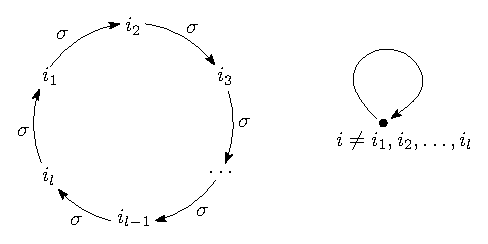
\includegraphics[width=0.55\textwidth]{AL1L7_1.eps}
	\caption{Орбита цикла $\sigma = (i_1,\dotsc,i_l)$.}
	\label{7_1}
\end{figure}
\textbf{Пример}: рассмотрим следующую подстановку:
$$
	\sigma = 
	\begin{pmatrix}
		1 & 2 & 3 & 4 & 5 \\
		4 & 2 & 5 & 3 & 1
	\end{pmatrix} \Rightarrow 1 \to 4 \to 3 \to 5 \to 1, \, 2 \to 2
$$
Следовательно, наша подстановка это цикл длины $4$. Запишем её в однорядной записи:
$$
	\sigma = (1435)
$$

\begin{rem}
	Циклы это простейшие, после тождественной, подстановки.
\end{rem}
\begin{defn}
	Два цикла $\sigma = (i_1\dotsc i_l)$ и $\pi = (j_1 \dotsc j_m)$ называются \uwave{независимыми}, если их орбиты не пересекаются:
	$$
		\{i_1, \dotsc, i_l\} \cap \{j_1, \dotsc, j_m\} = \VN
	$$
\end{defn}
\begin{prop}
	Независимые циклы коммутируют: если $\sigma$ и $\pi$ - независимы, то:
	$$
		\sigma{\cdot}\pi = \pi{\cdot}\sigma
	$$
\end{prop}
\begin{proof}
	Пусть $\sigma = (i_1\dotsc i_l)$ и $\pi = (j_1 \dotsc j_m)$ - независимы, тогда:
	$$
		\forall k \in \{i_1, \dotsc, i_l\}, \, \sigma{\cdot}\pi(k)= \sigma(\pi(k)) = \sigma(k) = \pi(\sigma(k)) = \pi{\cdot}\sigma(k)
	$$
	$$
		\forall k \in \{j_1, \dotsc, j_m\}, \, \sigma{\cdot}\pi(k) = \sigma(\pi(k)) = \pi(k) = \pi(\sigma(k)) = \pi{\cdot}\sigma(k)
	$$
	$$
		\forall k \in  \{1, \dotsc, n\} \setminus \left(\{i_1,\dotsc, i_l\} \cup \{j_1, \dotsc j_m\}\right) , \, \sigma{\cdot}\pi(k) = \sigma(\pi(k)) =  k = \pi(\sigma(k)) =\pi{\cdot}\sigma(k)
	$$
\end{proof}
\newpage
\section*{Разложение подстановки в попарно независимые циклы}
Перед формулировкой теоремы определим ряд понятий.
\begin{defn}
	Определим \uwave{возведение подстановок в степень} следующим образом:
	$$
		\sigma^k = \underbrace{\sigma{\cdot}\dotsc{\cdot}\sigma}_{k}, \, k \in \MN, \quad \sigma^k =\underbrace{\sigma^{-1}{\cdot}\dotsc{\cdot}\sigma^{-1}}_{|k| > 0}, \, k \in \MZ, \, k < 0, \quad \sigma^k = \VE, \, k = 0
	$$
\end{defn}

\begin{prop}(\textbf{свойства возведения подстановки в степень})
	\begin{enumerate}[label=(\arabic*)]
		\item $\sigma^k{\cdot}\sigma^l = \sigma^{k + l}, \, \forall k,l \in \MZ$;
		\item $(\sigma^k)^l = \sigma^{k{\cdot}l}, \, \forall k,l \in \MZ$;
	\end{enumerate}
\end{prop}

\begin{proof}\hfill
	\begin{enumerate}[label=(\arabic*)]
		\item Рассмотрим случаи:
		$$
			\forall k,l \in \MZ \colon k, l > 0 \Rightarrow \sigma^k{\cdot}\sigma^l = \underbrace{\sigma{\cdot}\dotsc{\cdot}\sigma}_{k}{\cdot}\underbrace{\sigma{\cdot}\dotsc{\cdot}\sigma}_{l} = \sigma^{k + l}
		$$
		$$
			\forall k,l \in \MZ  \colon k, l <  0 \Rightarrow \sigma^k{\cdot}\sigma^l = \underbrace{\sigma^{-1}{\cdot}\dotsc{\cdot}\sigma^{-1}}_{k}{\cdot}\underbrace{\sigma^{-1}{\cdot}\dotsc{\cdot}\sigma^{-1}}_{l} = \sigma^{k + l}
		$$
		$$
			\forall k,l \in \MZ \colon k < 0, l > 0 \Rightarrow \sigma^k{\cdot}\sigma^l = \underbrace{\sigma^{-1}{\cdot}\dotsc{\cdot}\sigma^{-1}}_{k}{\cdot}\underbrace{\sigma{\cdot}\dotsc{\cdot}\sigma}_{l} = \sigma^{\sgn{(k+l)}{\cdot}|k+l|} = \sigma^{k + l}
		$$
		\item Рассмотрим случаи:		
		$$
			l > 0  \Rightarrow (\sigma^k)^l = \underbrace{\sigma^k{\cdot}\dotsc{\cdot}\sigma^{k}}_{l} = \sigma^{k{\cdot}l}
		$$
		$$
			l < 0 \Rightarrow (\sigma^k)^l = \underbrace{\sigma^{-k}{\cdot}\dotsc{\cdot}\sigma^{-k}}_{|l|} = \sigma^{k{\cdot}l}
		$$
		$$
			l = 0\Rightarrow (\sigma^k)^0 = \VE
		$$
	\end{enumerate}
\end{proof}

\begin{defn}
	\uwave{Орбитой} числа $i \in \{1,\dotsc, n\}$ под действием $\sigma$ называется множество:
	$$
		O(i) = \{\sigma^{k}(i) \mid k \in \MZ\}
	$$
\end{defn}
\begin{prop}
	Орбита любого числа $i \in \{1,\dotsc, n\}$ есть следующее множество:
	$$
		O(i) = \{i, \sigma(i),\sigma^2(i), \dotsc \sigma^{m-1}(i)\}
	$$
	где $m$ такое наименьшее число, что $\sigma^m(i)= i$.
\end{prop}
\begin{proof}
	Все точки в одной орбите связаны следующим образом:
	$$
		\dotsc \to \sigma^{-2}(i) \to \sigma^{-1}(i) \to i = \sigma^{0}(i) \to \sigma(i) \to \sigma^{2}(i) \to \dotsc
	$$
	Цепочка бесконечная, но при этом орбита это конечное множество, поскольку $\{1,\dotsc,n\}$ - конечное множество чисел. Тогда: 
	$$
		\exists \, k \neq l \colon \sigma^k(i) = \sigma^l(i)
	$$ 
	Без ограничения общности, пусть $k > l$, тогда можем применить к левой и правой части $\sigma^{-l}$, тогда:
	$$
		\sigma^{k - l}(i) = \sigma^{0}(i) = \VE(i) = i, \, k -l > 0
	$$
	Поскольку существует $k -l > 0$ со свойством выше, то мы можем выбрать наименьшую положительную степень с таким свойством. Пусть $m > 0$ - наименьшая степень, такая что: $\sigma^m(i) = i$, тогда: 
	$$
		i \xrightarrow{\sigma} \sigma(i) \xrightarrow{\sigma} \sigma^2(i) \xrightarrow{\sigma} \dotsc \xrightarrow{\sigma} \sigma^m(i) \xrightarrow{\sigma} i \Rightarrow O(i) = \{i, \sigma(i),\sigma^2(i), \dotsc \sigma^{m-1}(i)\}
	$$
	$$
		O(i) = \{\sigma^{k}(i) \mid k \in \MZ\} =  \{i, \sigma(i),\sigma^2(i), \dotsc \sigma^{m-1}(i)\}
	$$
\end{proof}
\begin{prop}(\textbf{свойства орбит чисел})
	\begin{enumerate}[label=(\arabic*)]
		\item Разные орбиты не пересекаются;
		\item Орбиты образуют разбиение $\{1,\dotsc,n\}$ на попарно не пересекающиеся подмножества;
	\end{enumerate}
\end{prop}

\begin{proof}\hfill
	\begin{enumerate}[label=(\arabic*)]
		\item Пусть $O(i) \cap O(j) \neq \VN$, тогда $\exists \, k \in O(i) \cap O(j) \Rightarrow k = \sigma^p(i) = \sigma^q(j)$, следовательно, применив $\sigma^{-p}$:
		$$
			i = \sigma^{q - p}(j) \Rightarrow i \in O(j) \Rightarrow \forall l \in \MZ, \, \sigma^{l}(i) = \sigma^{l + q-p}(j) \in O(j) \Rightarrow O(i)\subseteq O(j)
		$$
		Аналогично, можно доказать обратное включение: $O(j) \subseteq O(i) \Rightarrow O(i) = O(j)$;
		\item Следует из того, что каждое число лежит в какой-нибудь орбите, например, в своей собственной: 	
		$$
			\forall i \in \{1,\dotsc, n\}, \, i \in O(i)
		$$
	\end{enumerate}
\end{proof}

\begin{theorem}
	Для любой подстановки $\sigma \in S_n$, существует разложение этой подстановки в произведение попарно независимых циклов $\sigma_1, \dotsc,\sigma_s$: 
	$$
		\sigma = \sigma_1{\cdot}\dotsc{\cdot}\sigma_s
	$$
	Причем это разложение единственно с точностью до перестановки сомножителей.
\end{theorem}
\begin{proof}\hfill
	\begin{enumerate}[label=\arabic*)]
		\item \textbf{Построение разложения $\sigma$ в произведение независимых циклов}: из свойств орбит числа получается, что: 
		$$
			\{1,\dotsc,n\} = O_1 \cup O_2 \cup \dotsc \cup O_s \cup O_{s+1} \cup \dotsc \cup O_t
		$$ 
		где орбиты $1,\dotsc, s$ состоят из нескольких чисел и орбиты $(s+1), \dotsc, t$ состоят из одного числа. Отсюда, мы получим:
		$$
			\sigma = (i_1^1 \dotsc i_{l_1}^1){\cdot}(i_1^2 \dotsc i_{l_2}^2){\cdot}\dotsc{\cdot}(i_1^s \dotsc i_{l_s}^s) = \sigma_1{\cdot}\dotsc{\cdot}\sigma_s
		$$
		они будут независимы, поскольку каждый цикл действует на своей орбите, а орбиты не пересекаются. Таким образом, мы получили разложение;
		
		\item \textbf{Единственность}: пусть $\sigma = \sigma_1{\cdot}\sigma_2{\cdot}\dotsc{\cdot}\sigma_s$, где $\sigma_i$ - попарно независимые циклы: 
		$$
			\sigma_1 = (i_1^1 \dotsc i_{l_1}^1), \dotsc, \sigma_s =(i_1^s,\dotsc,i_{l_s}^s)
		$$
		Тогда $\sigma$ действует на множество чисел $\{1,\dotsc,n\}$ по схеме:
		$$
			\forall i_j^k \in \{1,\dotsc, n\}, \, \sigma(i_j^k) = \sigma_k(i_j^k)
		$$ 
		Следовательно, орбиты подстановки $\sigma$ в $\{1,\dotsc,n\}$ - это орбиты циклов $\sigma_1,\dotsc,\sigma_s$, потому что каждое из чисел попадает в одну из орбит и на это число будет действовать только соответствующий цикл, остальные циклы будут оставлять это число на месте.	Также заметим, что по $\sigma$ можно однозначно восстановить орбиты независимых циклов $\sigma_1, \dotsc, \sigma_s$ в разложении $\sigma \Rightarrow$ можно восстановить и сами циклы $\sigma_i$, потому что на своей орбите $\sigma_i$ действует также как вся подстановка $\sigma$.
		
		Таким образом, зная подстановку $\sigma$ мы можем однозначно восстановить орбиты этих циклов. А зная эти орбиты и подстановку $\sigma$ мы можем восстановить порядок перестановки элементов в орбите, то есть восстановить сами циклы;
	\end{enumerate}
\end{proof}

\textbf{Пример}: 
$$
	\sigma = 
	\begin{pmatrix}
		1 & 2 & 3 & 4 & 5 & 6 & 7 & 8\\
		4 & 7 & 5 & 3 & 1 & 6 & 8 & 2
	\end{pmatrix}
$$
$$
	1 \to 4 \to 3 \to 5 \to 1, \quad 2 \to 7 \to 8 \to 2, \quad 6 \to 6 \Rightarrow
$$
$$
	\Rightarrow \sigma = (1435){\cdot}(278) = \sigma_1{\cdot}\sigma_2
$$
Получили циклы длины $4$, $3$ и стационарную точку.

\end{document}